\begin{question}
\noindent Triangle $A$ has vertices at $(-5, 1)$, $(-5, 4)$ and $(-2, 1)$.
Triangle $B$ has vertices at $(2, -1)$, $(2, -4)$ and $(5, -1)$.

\begin{center}
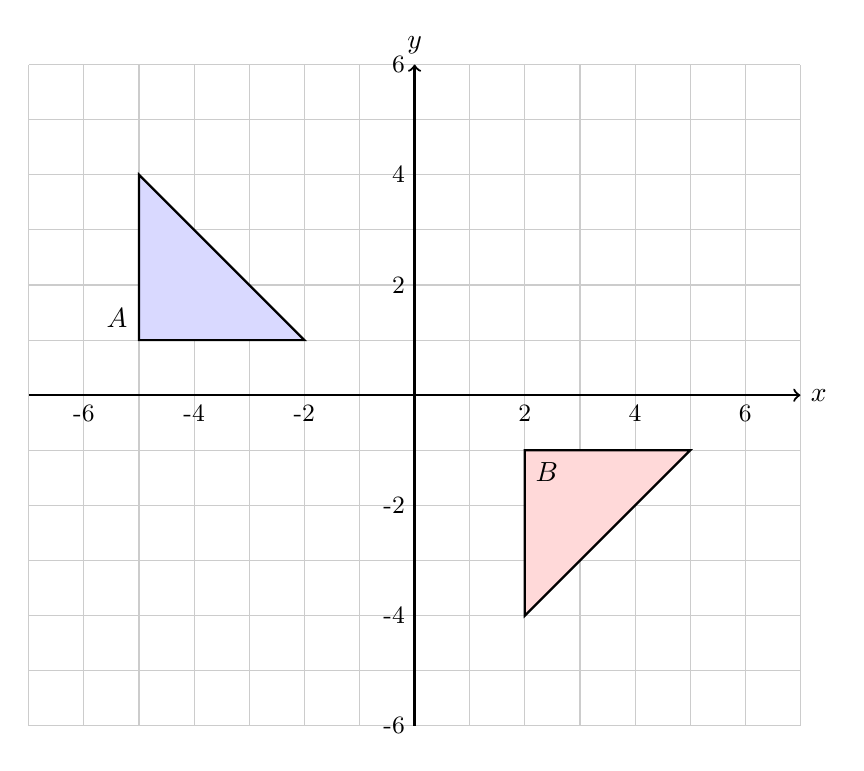
\begin{tikzpicture}[scale=0.7]
    % Grid
    \draw[step=1cm, gray!40, thin] (-7,-6) grid (7,6);

    % Axes
    \draw[thick, ->] (-7,0) -- (7,0) node[right]{$x$};
    \draw[thick, ->] (0,-6) -- (0,6) node[above]{$y$};

    % Axis tick labels
    \foreach \x in {-6,-4,-2,2,4,6}
        \node[below] at (\x,0) {\small \x};
    \foreach \y in {-6,-4,-2,2,4,6}
        \node[left] at (0,\y) {\small \y};

    % Triangle A
    \draw[thick, fill=blue!15] (-5,1) -- (-5,4) -- (-2,1) -- cycle;
    \node at (-5.4,1.4) {$A$};

    % Triangle B
    \draw[thick, fill=red!15] (2,-1) -- (2,-4) -- (5,-1) -- cycle;
    \node at (2.4,-1.4) {$B$};

\end{tikzpicture}
\end{center}

\noindent Describe fully the single transformation that maps triangle $A$ onto triangle $B$.

\vspace{4cm}
\begin{flushright}
    \answerlines{3}{3}
\end{flushright}
\end{question}
